\subsection{Pipelining}

Multi-cycle processors are an improvement over single-cycles processors, but they still spend a great amount of time only doing one thing.
Pipelining is a technique that dramaticly increases the throughput of a multi-cycle processor by allowing different stages of different instructions to execute at the same time.

The execution of an instruction is usually split into five stages:
Fetch, Decode, Execute, Memory and Writeback. 
This means that 5 different instructions can be executed in parallell,
one in each stage, as seen below in figure \ref{fig:pipeline}.
\footnote{
    The number of stages can vary.
    Some versions of Intel Pentium 4 had a whopping 31-stage pipeline.
    \cite{wiki-pentium4}
}

\begin{figure}[ht]
    \centering
    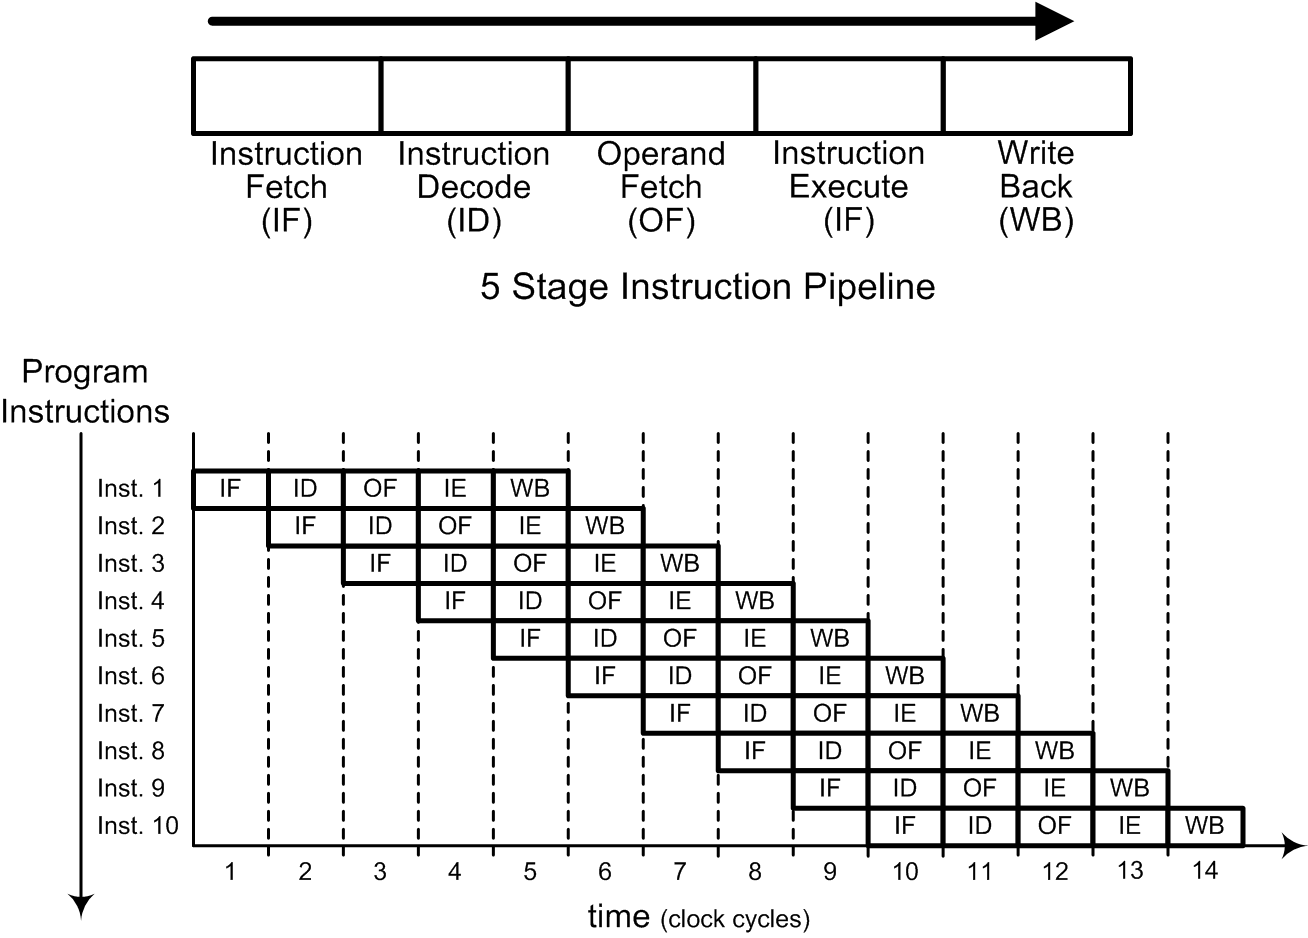
\includegraphics[width=\textwidth]{figures/pipeline2.png}
    \caption{A pipeline during execution} 
    \label{fig:pipeline}
\end{figure}

\subsubsection*{Hazards}
However, pipelining is not that simple. Problems can occur when one instruction
is dependent on the result from a previous instruction which has not yet fully completed.
This can be solved by inserting stall instructions called nops when there are dependencies,
but this reduces performance. Another solution is to perform instruction reordering
but that leaves extra work for the programmer.
However, this issue can be circumvented by sending the results from previous, not
yet completed stages to following stages.
This is called forwarding, and will prevent the need for nops in almost all cases.
\cite{hazards-lecture}

\subsection{Optimization}

\subsubsection*{Forwarding}
Instead of inserting pipeline bubbles, forwarding can be implemented. To forward
is to send the result of an instruction back in the pipeline to an earlier
dependent step. A trivial example of this can be

\begin{verbatim}
a = 1 + 1
b = a + 1
\end{verbatim}

as \textit{b} is dependent on \textit{a}, and that instruction needs to be done.
By sending \textit{a} back, the second instruction can be completed in time.


\subsubsection*{Branch prediction}
In the case of branching, the processor can't add the next instruction to the
pipeline, as it isn't sure of what instruction is the next. To solve this
problem, branch prediction tries to guess whether or not a branch will be
followed. This allows to then find the next instruction, and thus add the next
instruction to the pipeline.


\subsubsection*{Flushing}
If a branch is taken, but was assumed not, the instruction in the pipeline must
be discarded. This is called flushing, and is done by inserting NOP instructions
instead of instructions that should be executed.
